
\documentclass[titlepage]{scrartcl}
\usepackage{enumitem}
\usepackage[british]{babel}
\usepackage[style=apa, backend=biber]{biblatex}
\DeclareLanguageMapping{british}{british-apa}
\usepackage{url}
\usepackage{float}
\restylefloat{table}
\usepackage{perpage}
\MakePerPage{footnote}
\usepackage{abstract}
\usepackage{graphicx}

\usepackage[T1]{fontenc}
\usepackage[utf8]{inputenc}
\usepackage{blindtext}
\setkomafont{disposition}{\normalfont\bfseries}


\graphicspath{
    {./resources/},
}
\addbibresource{~/PerryPerrySource/LaTeX/DSP_Bibliography.bib}

\newsavebox{\abstractbox}
\renewenvironment{abstract}
  {\begin{lrbox}{0}\begin{minipage}{\textwidth}
   \begin{center}\normalfont\sectfont\abstractname\end{center}\quotation}
  {\endquotation\end{minipage}\end{lrbox}%
   \global\setbox\abstractbox=\box0 }

\usepackage{etoolbox}
\makeatletter
\expandafter\patchcmd\csname\string\maketitle\endcsname
  {\vskip\z@\@plus3fill}
  {\vskip\z@\@plus2fill\box\abstractbox\vskip\z@\@plus1fill}
  {}{}
\makeatother

\DeclareCiteCommand{\citeyearpar}
    {}
    {\mkbibparens{\bibhyperref{\printdate}}}
    {\multicitedelim}
    {}

\begin{document}
    \title{DSP Assignment 2\\Digital Audio Effects Implementation}
    \subtitle{\LARGE{Technical Report}}
    \author{Sam Perry\\U1265119}
    \date{}

    \begin{abstract}
        This report outlines the implementation, testing and evaluation of
        three real-time audio effects using the dsPIC 30F4013 digital signal
        processor.  Design choices, system specification, and final results
        are analysed.\\
        System specification is compared with alternative chips to understand
        the quality of the processor in relation to the state of DSP
        technology.\\
        Design choices are compared to choices made in previous work to outline
        the changes required to implement such effects outside of
        unlimited resource systems.\\
        Final system performance is then discussed to determine further
        changes that could be made to improve performance.
    \end{abstract}

    \maketitle


    \section{Background/Literature:\\Digital Signal Processor/Microcontroller
    Overview}
    A digital signal processor (DSP) is form of specialized microprocessor
    designed specifically for the processing of signals (such as audio signals
    in this case).~\parencite[p.11-12]{libtak2006ieh}. The DSP is used as part
    of a microcontroller that provides an interface for components such as
    Memory, data IO and peripherals that form the signal processing system.
    When considering the quality of a DSP system, there are many component
    specifications to consider, that contribute to the overall performance of
    the system. These include:
    \begin{itemize}
        \item CPU
        \item Memory
        \item System bus
        \item Bit depth
        \item Samplerate
        \item D/A \& A/D converters
    \end{itemize}

    In order to understand the specification of the dsPIC in relation to the
    standard of DSPs available, it will be compared to three other digital signal
    processors:
    \begin{itemize}
        \item Texas Instruments TMS320F2806x
        \item Freescale 56F8025
        \item Analog Devices ADSP-2126x
    \end{itemize}

    \subsection{General Computing Factors}
    Factors such as memory and CPU speed are factors that affect all computing
    systems. These address the systems ability to perform calculations and
    handle data.

    \subsubsection{Memory}
    There are two types of memory that constitute the total memory of a
    microcontroller: program memory and data memory.

    \paragraph{Program Memory}~\\
    Most modern microcontrollers use flash memory for the storage of code
    executed at runtime. This is known as ROM (read-only memory) and may be
    reffered to as the ``program memory''. The size of this memory determines
    the amount of code that can be stored at any one time in the processor.
    This has implications with regaurds to the complexity of the program as
    insufficient program memory will limit the number of instructions that can
    be used for programming.

    \paragraph{Data Memory}~\\
    RAM (random-access memory) is volatile memory that is used for storing data
    used when executing instructions. Unlike ROM memory, RAM can be both read
    from and written to at runtime and is used for the storage of data that can
    change as instructions are executed. This is used for the storage of data
    such as audio buffer and parameter variables. The amount of RAM available
    determines the maximum size of data such as buffers for audio delays. The
    speed of the RAM is also integral to the overall performance of the system
    as sufficient speed is required to read and write buffers as instructions
    are executed by the CPU (see section \ref{CPU})

    \subsubsection{System Bus}
    The system bus handles data IO between components such as the CPU
    and memory. For performance comparisson, the system bus's data width is
    used to determine the maximum amount of memory that the CPU is able to
    write directly to memory. 
    For example a 16BIT system can support a maximum of $2^{16}$ memory
    addresses. This equals a maximum memory size of 64Kb of memory directly
    accessible by the CPU. However, a 32BIT system can support $2^{32}$ memory
    addresses which results in ~4GB of potential memory.
    When analysing specifications of DSP systems it is important to seperate
    the processing architechuture from the bit depth of the DSP components as
    they affect different aspects of the system.

    \subsubsection{CPU}\label{CPU}
    The CPU (Central Processing Unit) is the component that executes
    instructions and performs calculations on data. The speed at which the CPU
    can execute instructions and store results is critical to the performance
    of the system.

    \paragraph{Clock Speed}~\\
    Measured in cycles per second (Hz), the clock speed defines the number of
    calculations that can be performed per second. A higher clock speed
    indicates a higher number of calculations performed per second. This is
    particularly significant in realtime DSP application as a sufficient number
    of calculations must be performed in a set period of time in order to
    process audio as quickly as it is provided to the system.  If the clock
    speed is not sufficient, this may result in instructions being missed due
    to an interupt before the processor has been able to complete them. This
    can create in artefacts in output audio and create unexpected results.

    \paragraph{Architecture}~\\
    The CPU architecture refers to the design of memory units and bus layouts.
    The most common designs are von Neumann and Harvard architectures. The von
    Neumann architecture combines program and memory data, allowing only serial
    access of memory. By seperrating program and data memory, the Harvard
    architecture allows for simulataneous access of data and program memory,
    making it the more efficient of the two designs.
    \begin{figure}[H]
        \caption{von Neumann CPU architecture}
        \makebox[\textwidth]{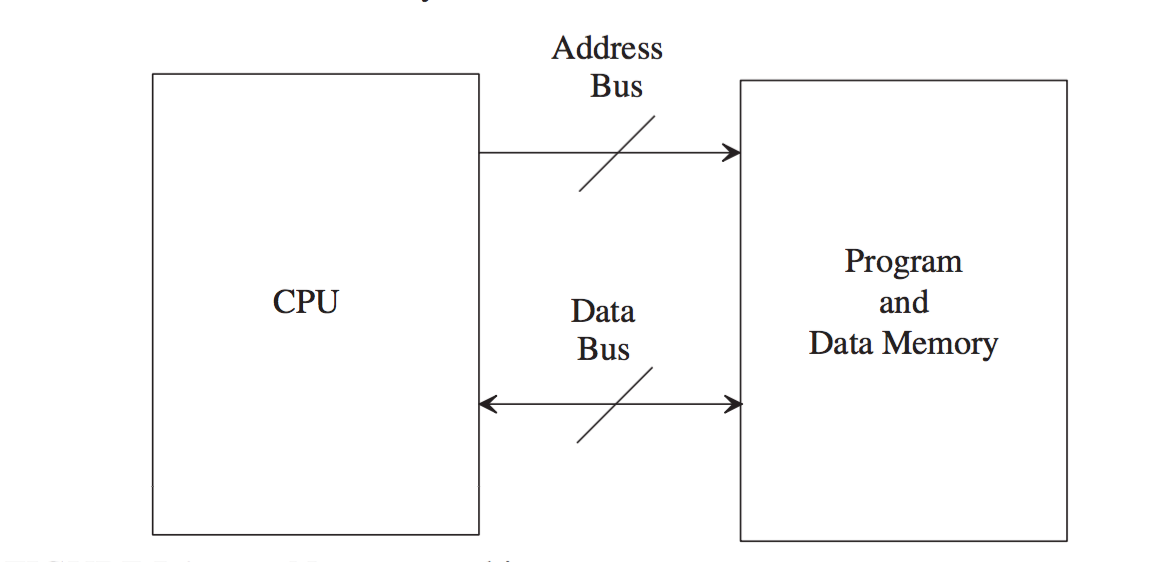
\includegraphics[width=0.75\textwidth]{neumann}}
    \end{figure}
    \begin{figure}[H]
        \caption{Harvard CPU architecture}
        \makebox[\textwidth]{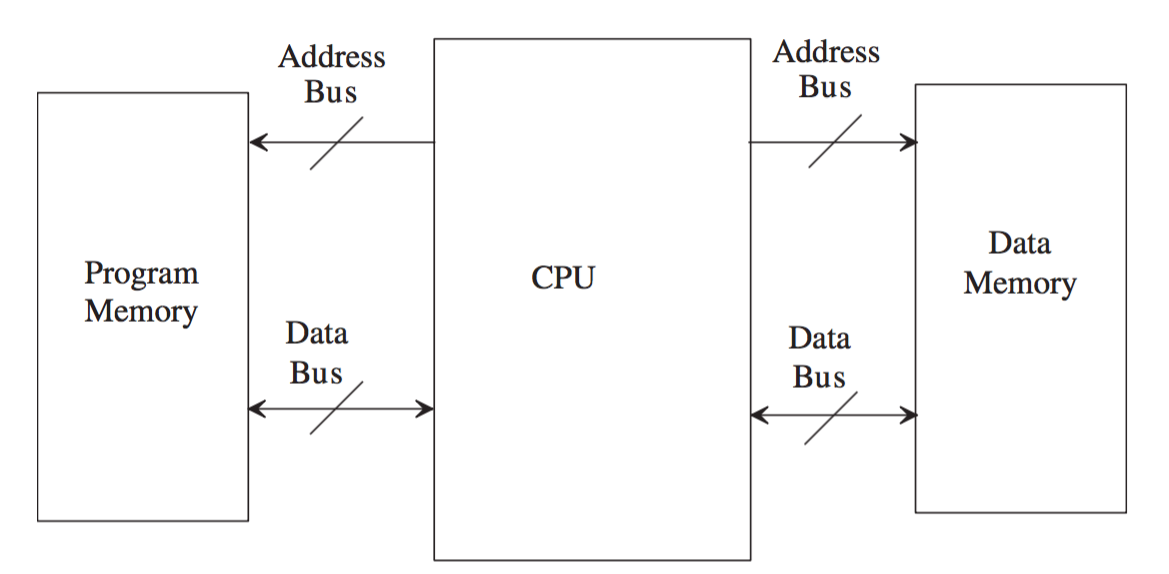
\includegraphics[width=0.75\textwidth]{harvard}}
    \end{figure}
    \newpage 
    \section{DSP Specific Factors}
    DSP specific factors relate to components specically affecting the systems
    ability to handle audio signals. These will determine the quality of audio
    manipulation and affect the computational requirements for the system.

    \subsection{A/D \& D/A Converters}
    A/D and D/A converters are required for audio input and output. Depending
    on the microcontroller used, these may intergrated in the main circuit
    board or available as peripherals that can be attached via ports (as is the
    case for the PIC24 board used). The quality and accuracy of these
    converters will clearly have an effect on the audio output and using
    converters that can perform as transparently as possible is essential for a
    high quality system.
    
    \subsection{Samplerate}
    The samplerate defines the frequency at which a measurement will be taken
    from the input audio. This is significant due to the quantity of
    information returned from the A/D converter for processing. Higher sample
    rates generates more measurements per second and thus requires more values
    to be computed per second.
    \begin{figure}[H]
        \caption{Illustration of sine wave sampling}
        \makebox[\textwidth]{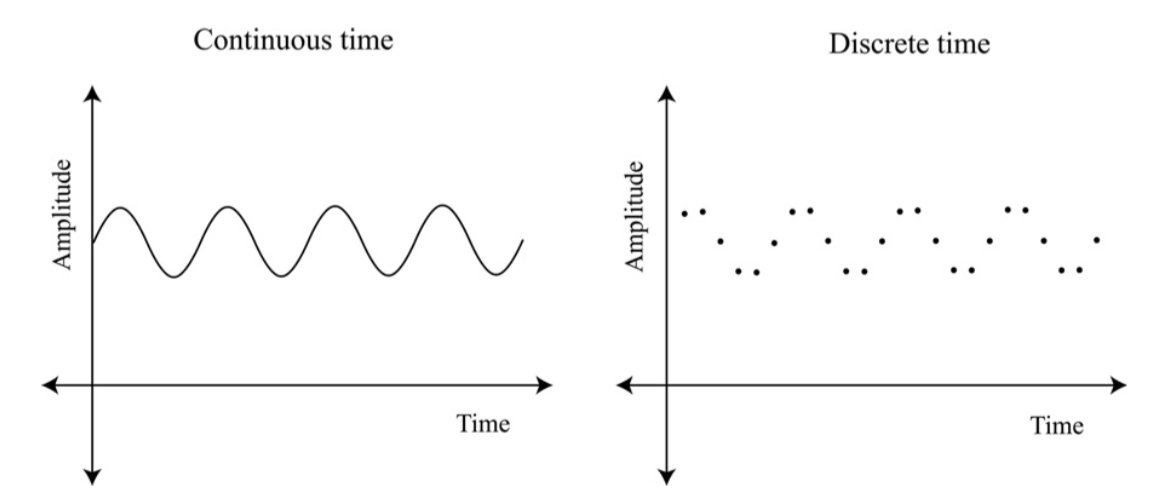
\includegraphics[width=\textwidth]{quantization}}
    \end{figure}
    \begin{figure}[H]
        \caption{Illustration of quantization error resulting from a low sample
        rate.}
        \makebox[\textwidth]{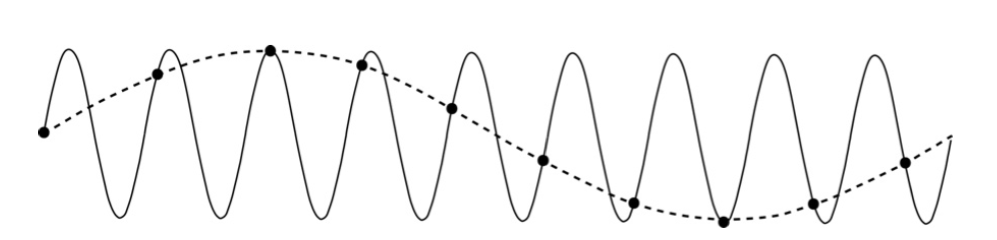
\includegraphics[width=\textwidth]{sampling_error}}
    \end{figure}

    \subsection{Bit Depth}
    The audio bit depth determines the accuracy to which amplitudes can be
    differentiated. Higher bit depths result in a higher dynamic range in the
    signal. This has implications for the converters as higher bit rates
    require higher accuracy in generating values for each sample.

    \section{Design/Analysis}
    Effect implementation wase largely dicatated by the limitations of the
    dsPIC. As the device had sever memory and processing limitations, it was
    not possible to create effects to the standard of the first assignment. As
    a result effects were created to emulate the perceptual effect of an echo,
    reverb and chorus under these limitations.

    \subsection{Echo}
    The echo was implemented using a single tap FIR filter. This was intended
    to maximise available memory for the delay time. Through stripping out all
    unnessesary features, a maximum delay size of 700 samples was acheived with
    the addition of two UI switches that could be used for increasing and
    decreasing delay size at runtime.
    At a samplerate of 8Khz, this allowed for a single delay of \textgreater50ms defined
    as the minimum for the definition of an echo
    by Z{\"o}lzer~\citeyearpar[p.]{zolzer2011dafx}

    \subsection{Chorus}
    To emulate the multiple instrument effect created by a chorus, three delays
    of variable size were used. This created 3 phase shifted versions of the
    original signal which creates the perception of multiple instruments. The
    delay time modulation was not possible due to the computational power
    required to implement this for modulating a delay time on a sample by
    sample basis.

    \subsection{Reverb}
    The reverb implementation involved a combination of an FIR and IIR filter
    as defined by Z{\"o}lzer~\citeyearpar[p.]{zolzer2011dafx}. This performed
    poorly when compared to the moorer reverb structure used in assignment 1,
    however the complexity of such a structure would require superior
    performance in almost all aspects of the system.
    The design used created a delayed echo that could act as a crude reverb.

    \subsection{User Interface}
    The UI was designed using eight switches and the LCD to create a
    navigatable menu that can be used for the section of effect, effect
    parameters and voculme control. The effect parameter menu is able to update
    it's items dynamically based on the active effects. The desired effect can
    then be selected by cycling through using repeated presses of the effects
    menu button. Parameter varaibles can then be increased and decreased for
    the selected effect using two switches.\\
    It was not possible to use the UI in conjunction with any actual audio
    effect as proper threading of the menu alongside the DSP process was not
    possible. Having the menu run in the same thread as signal processing
    forced menu logic to complete at signal rate. When this did not occur this
    would create unexpected results and graphical error in the LCD as logic was
    not completed fully. As a result, the project presented is a prototype to
    demonstrate possibilities given a capable system.

    \section{Results}
    The results of real-time system implementation section should include:\\
        Implementation on dsPIC based system\\
        Testing and evaluation of the artificial reverberation system\\
        Expected frequecy range based on samplerate
        \subsection{Echo}
        Maxmum  achieved.
        Audio sound quality acheived
        \subsection{Chorus}
        Maximum delay buffer size
        Audio sound quality acheived
        \subsection{Reverb}
        Audio sound quality acheived

        
    \section{Further Work}
    The student should discuss the limitations of the system and how it could be developed further

    \section{Conclusions}
    The conclusion section should include:\\
    dsPIC30F4013 not fit for the purpose of this task.
        Critical discussion about the system, (did it work? if not, why
        not?).\\
        Statement of what the student learned from the exercise.\\

    \printbibliography

\end{document}
